\subsection{Definition and motivation}
Topology Optimization describes the process of finding the optimal distribution of a limited amount of material for a given area or volume based on a predefined constraint/minimization problem. Possible optimization goals are for example:
\begin{itemize}
\item \textbf{Minimum compliance} which seeks to find the optimal distribution of material that returns the stiffest possible structure. The structure is thereby subjected to loads (forces) and supports (boundary conditions). By maximizing the stiffness, we minimize the compliance.
\item \textbf{Heat conduction} tries to optimize the domain of a conductive material with respect to conductivity for the purpose of heat transfer. This maximization problem is the same as minimizing the temperature gradient over the domain-- a poor conductor will create a large gradient.
\item \textbf{Mechanism synthesis}' objective is to obtain a device that can convert an input displacement in one location to an output displacement in another location. Topology Optimization hereby seeks the optimal design which maximizes the output force for a given input or, respectively, minimizes the input force for a given output.
\end{itemize}


As one can imagine by this short list of optimization goals, Topology Optimization has a wide field of possible applications. Hence, it has become a well established technology used by engineers in the fields of aeronautics, civil, materials, mechanical and structural optimization. Furthermore, the rising significance of 3D-printers in industry, the realisation of computed optimized designs is now much easier.

\subsection{Theory}
%Maybe a little theory here about how topology optimization actually works

\subsection{ToPy}
ToPy \cite{ToPy} is a python library/program, written by William Hunter and documented in \cite{Hunter2009}. It is based on the 99-line Matlab code by Sigmund's for minimum compliance. The program can optimize the three above named problem types, minimum compliance, heat conduction and mechanism synthesis-- in 2D as well as 3D. It uses available open source python software, as for example Pysparse and Numpy, leading to improved speed, porta- and scalability. The whole program is steered by an input file which-- with the help of the documentation-- is straightforward to use and easy to adapt. 

\subsection{Implementation}
In terms of our implementation, we use ToPy as a blackbox topology optimizer. This means, we launch the program with an input file based on our scenario, let ToPy run and proceed by working with the output of ToPy. The intention is to touch the solver itself as less as possible to be able to just plug in different solvers later on. Implementation-wise that means, that we wrote a program which takes as input a voxelized CAD design in, for example, stl-format and outputs a tpd-file which can be used by ToPy. Results of the process can be seen in figure \ref{fig: topyStar}. Here, a star was given as input from a stl-file. We fixed the voxels in the corners of the structure, while we set a load in the middle, pointing into the structure. As can be seen, the optimization process "cuts" away unnecessary material in-between the corners and even in the middle of the material and returns stiff structure for a minimal amount of material. (maybe a bit wishy washy here)
\begin{figure}
\centering
\begin{subfigure}{
  
\includegraphics[width=.2\linewidth]{Pictures/TopOp/Star_Optimized0_Trans.png}}
\end{subfigure}%
\begin{subfigure}{
  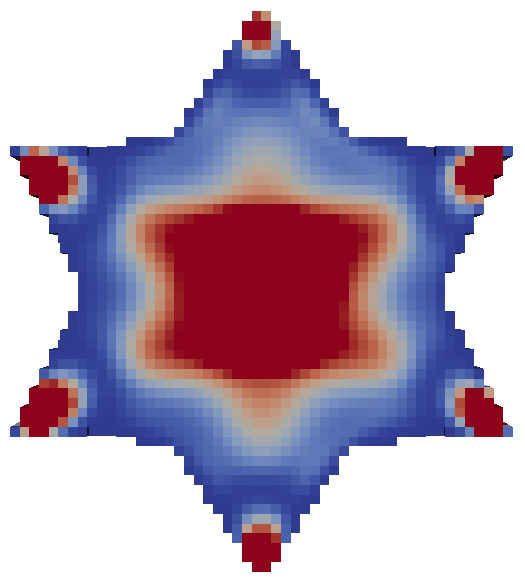
\includegraphics[width=.2\linewidth]{Pictures/TopOp/Star_Optimized2_Trans.png}}
\end{subfigure}
\begin{subfigure}{
  
\includegraphics[width=.2\linewidth]{Pictures/TopOp/Star_Optimized4_Trans.png}}
\end{subfigure}
\begin{subfigure}{
  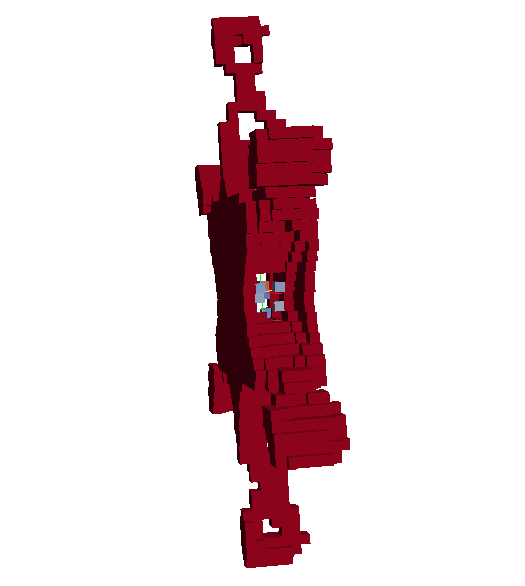
\includegraphics[width=.2\linewidth]{Pictures/TopOp/Star_Optimized5_Trans.png}}
\end{subfigure}
\caption{Topology Optimization with minimum compliance of a star structure, given by an stl-file. The fixtures were applied in the corners of the star, while a load was set in the middle.}
\label{fig: topyStar}
\end{figure}
